\section{La Paz, Humahuaca et Salaar}

Date: 05/11/2009

\begin{multicols}{2}

Hola señioritas y señors.

Nous revoici réunis pour la suite de mon voyage, je vous emmène aujourd'hui à La Paz, capitale de la Bolivie où nous feront un petit tour de VTT. Nous descendrons ensuite beaucoup plus au sud, vers l'Argentine puis nous remonterons petit à petit, a Tupiza pour aller voir le Salaar de Uyuni qui est un magnifique désert de sel, nous prendrons ensuite le train pour Oruro et nous terminerons à Cochabamba, où je suis aujourd'hui.

Je vous ai donc laissés à Copacabana, au bord du lac Titicaca. C'est donc parti pour chercher un bus pour La Paz, qui est à 3h de transport. La portion Copacabana/La Paz est connue pour avoir eu pas mal de détournements et détroussements de touristes, je m'assure donc bien d'être sur une ligne régulière, même si je prend un petit collectivo (minivan). L'arrivée sur La Paz est assez impressionnante, car cette ville est située dans une espèce de fosse dont on ne voit rien avant d'arriver au bord de la falaise. Voici une petite photo de cette ville dont on m'avait tant parlé.

\hspace*{-0.65cm}
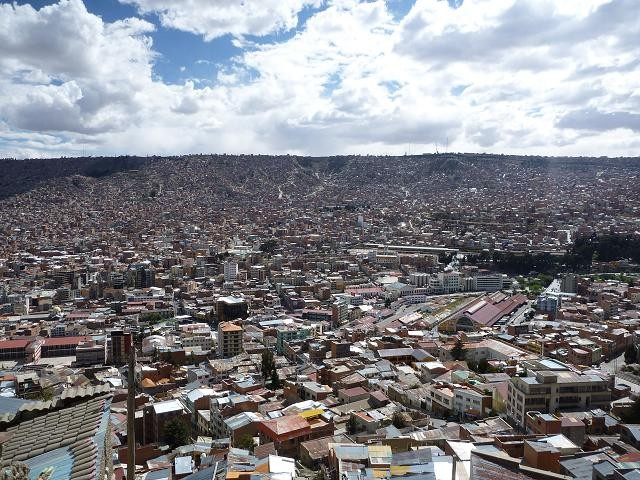
\includegraphics[width=4.8cm]{articles/La-paz-humahuaca-et-salaar/1257387232lefu.jpg}
La Paz.

La Paz est orientée autour d'une grande avenue centrale, qui change 3 fois de nom sur sa longueur, et qui permet de ne jamais se perdre, l'essentiel étant de revenir dans cette avenue si vous avez un doute sur votre position. Comme partout au Pérou ou en Bolivie, il est très facile de se déplacer grâce à des collectivos qui n'arrêtent pas d'aller et venir dans toutes les grandes rues, c'est surtout pratique pour monter, et à La Paz, c'est pas du luxe..

Bon, cette ville est sympa, mais elle me sera surtout utile pour faire un peu de shopping pas cher avant de retourner au Pérou. Pour l'heure, nous allons faire un petit tour de VTT sur la route la plus dangereuse du monde. La route de La Paz à Coroico, longue d'un peu plus de 70km a en effet cette spécificité, car par endroits elle est large de seulement 3,20m et borde un precipice de 600m.. Depuis deux ans une autre route de l'autre coté de la montagne a été ouverte, beaucoup plus sécurisée, et l'ancienne est maintenant devenue le terrain de jeu de tous les amateurs de VTT. Ce qui est super dangereux en voiture devient beaucoup plus sécurisant en VTT et on ressort grisé par la vitesse, mais non par le risque que l'on vient de cotoyer. En 5 heures, nous avons dévalé 3400m de dénivelé sans quasiment jamais avoir à pédaler, que du bonheur..

\hspace*{-0.65cm}
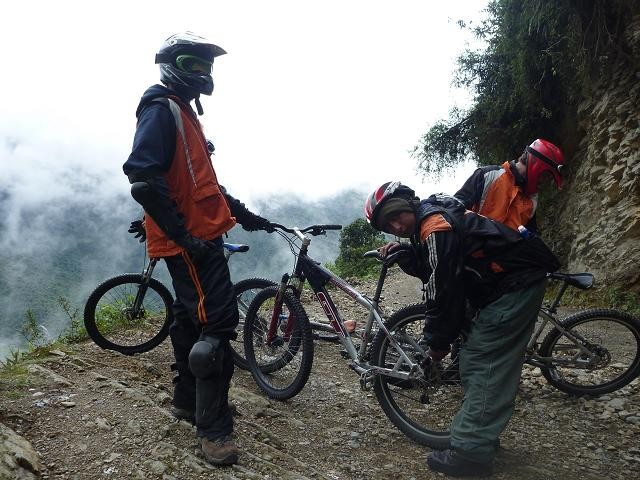
\includegraphics[width=4.8cm]{articles/La-paz-humahuaca-et-salaar/1257387311RBTU.jpg}
La route de la mort à vélo, de La Paz à Coroico.

Voici une photo de la route en question.

\hspace*{-0.65cm}
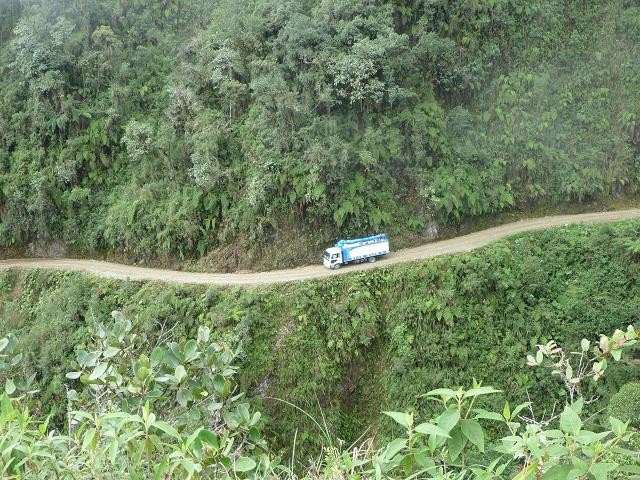
\includegraphics[width=4.8cm]{articles/La-paz-humahuaca-et-salaar/1257387218mz18.jpg}
Sympa cette petite route :)

Allez c'est parti, on lève l'ancre direction le Sud. Je prend un bus pour Tupiza dans le but de faire un tour dans le Salaar de Uyuni. Et zou, je m'embarque à 19h pour un voyage de 17h de bus sur route, puis sur piste cahoteuse le long de la route en construction. Vous n'imaginez même pas par où un bus à deux étages est capable de passer lorsqu'il a un bon pilote et de bons amortisseurs !!

\hspace*{-0.65cm}
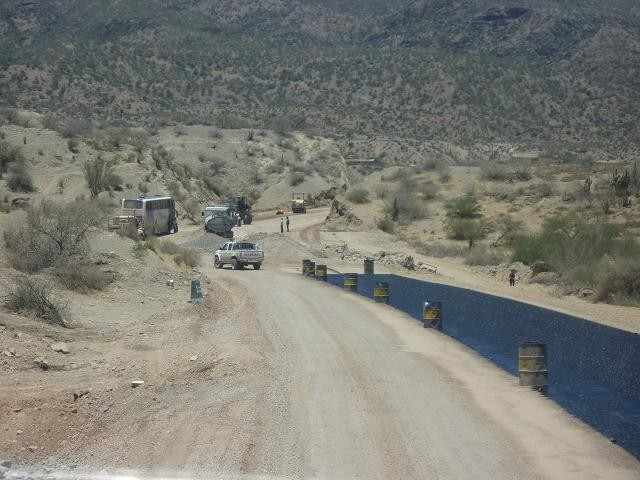
\includegraphics[width=4.8cm]{articles/La-paz-humahuaca-et-salaar/1257387196swjJ.jpg}
Bloqués 2h en attendant que le bitume sèche.

\hspace*{-0.65cm}
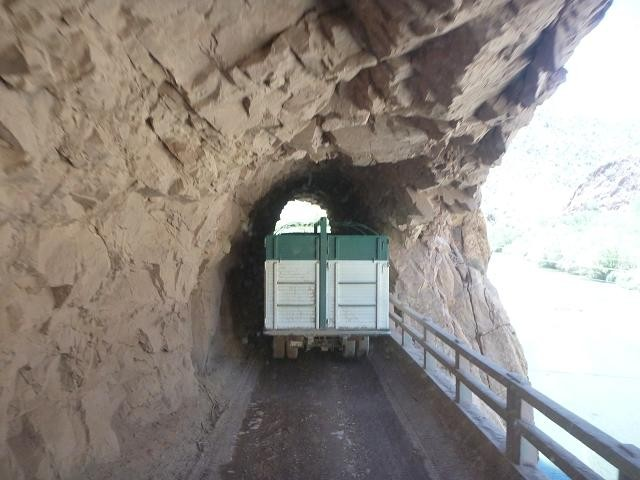
\includegraphics[width=4.8cm]{articles/La-paz-humahuaca-et-salaar/1257387183J7sM.jpg}
A toute blinde en bus à 2 étages dans les tunnels.

En discutant dans le bus, je m'aperçoie qu'il va jusque la frontière Argentine, soit 3h de plus. Ca me fait hésiter à continuer, ben oui on m'a tellement parlé du steak Argentin que je me dit que ce serait bien de tenter le coup. Ca y est on est a Tupiza, je sort du bus croyant qu'il fait une halte de 3h avant de repartir, j'ai donc 3h heure pour choisir si je continu ou pas. Mais que nenni !! A peine dehors le bus redémarre, la halte n'était que de quelques minutes. Mon sac est encore dans la soute, j'ai juste le temps de remonter, mais il n'est deja plus question de ré-ouvrir la soute. C'est donc reparti pour la frontière Argentine, le choix s'est fait sans moi. A vrai dire je ne sais pas vraiment si c'est une réélle incomprehension ou alors une blague du chauffeur voyant que j'hésitait, toujours est-il que me voila embarqué pour 3h de route en plus jusqu'à la frontière avec l'Argentine, à Villazon. Là je descend du bus et je suis subitement pris d'une poussée de fièvre de fou accompagnée d'un petit mal de tête des familles, je suis obligé de me poser dans un petit boui boui pour quelques heures, à boire du mate de coca (the aux feuilles de coca, sensé aider dans ces cas là). Puis je passe la frontiere, émigration puis immigration un petit taco pour aller au bus terminal et je prend un ticket pour Humahuaca, petite ville que m'a conseillée une des passagères du bus bolivien. Et hop, +3h de bus. Si on compte bien ça me fait alors 23h de bus et une tourista corsée, j'aime mieux vous dire que j'en menait pas large à ce moment là.

Ce dernier trajet de 3h a été marqué par deux arrêts par les flics locaux pour contrôle anti narcotiques. Le premier se solde par une montée des flics dans le bus, un bref regard et une discussion avec le chauffeur et tout est réglé, nous embarquerons 5 passagers à l'oeuil mais le contrôle n'aura pas lieu. Le deuxième est plus serieux. Tout le monde doit descendre, on récupère chacun nos sac dans la soute et on se met en file, une pour les hommes et une pour les femmes avec au bout un flic qui fouille les sacs et les personnes. Je ne tient qu'à peine debout, j'ai du mal à déplacer mon sac, je me dit qu'il vont me prendre pour un gros toxico. A ce moment un nouveau flic arrive, il voit ma tête de cachet d'aspirine et me prend à part, je me dit "meeerde, c'est parti pour les emmerdes", même si j'ai rien à me reprocher. On va dans leur maisonnettes, je pose mon sac sur la table et vait pour l'ouvrir, il m'arrête direct, me demande mon passeport, y jette a peine un oeuil et me dit que c'est bon, je peux sortir et passer à travers le contrôle. C'est donc officiel, en Argentine on peut être trafiquant de drogue, du moment qu'on a un passeport de gringo, les emmerdes sont évitées.

J'arrive enfin à Humahuaca, province de Jujuy (prononcez coucouille..) où je trouve un petit hôtel tenu par Hector qui fera tout pour que je me sente bien et me requinque. Un grand merci à Hector.

\hspace*{-0.65cm}
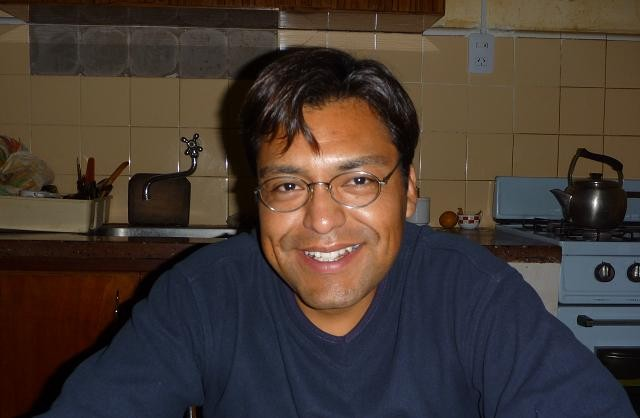
\includegraphics[width=4.8cm]{articles/La-paz-humahuaca-et-salaar/1257388208hISG.jpg}
"Hector, mon sauveur de Humahuaca"

Les environs de Humahuaca.

\hspace*{-0.65cm}
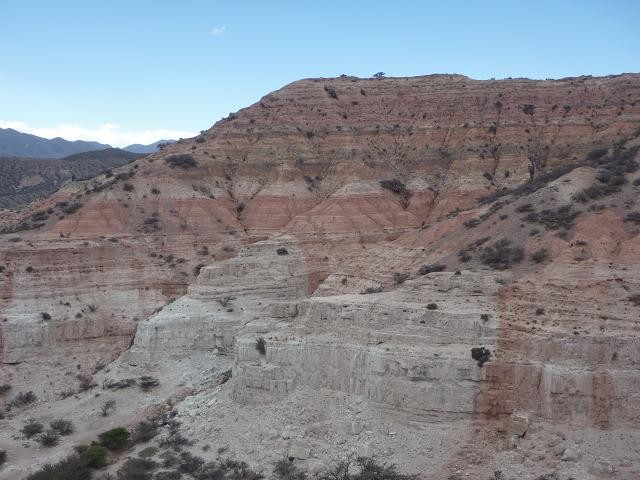
\includegraphics[width=4.8cm]{articles/La-paz-humahuaca-et-salaar/125738819811hb.jpg}
Les alentours de Humahuaca.

Une rue de la ville le soir.

\hspace*{-0.65cm}
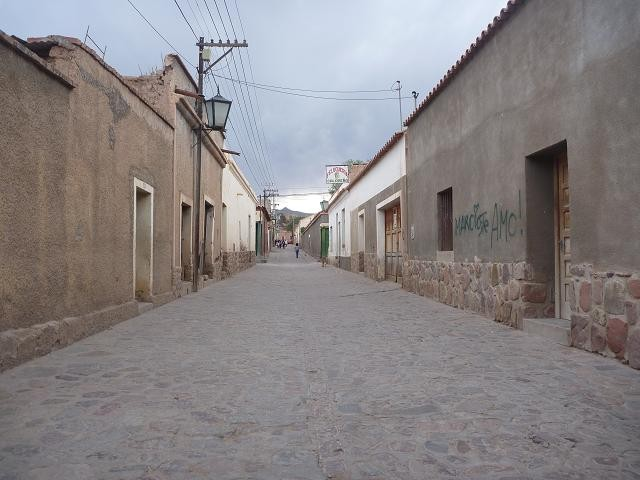
\includegraphics[width=4.8cm]{articles/La-paz-humahuaca-et-salaar/1257387531xqvF.jpg}
Les rues du centre ville.

Après deux jours à me remettre debout, et après avoir mangé un excellent steak Argentin, je repars de Humahuaca pour refaire la route vers Tupiza et partir vers le Salaar de Uyuni. J'arrive le soir à Tupiza, et tous les tours partant le lendemain sont pleins, dans toutes les agences où je vais. Qu'à cela ne tienne, je trouve deux anglais qui sont dans le même cas que moi, puis nous allons voir les agences en leur disant que nous sommes 3, que ça vaut le coup de créer un nouveau groupe rien que pour nous. C'est donc bon pour le lendemain matin, 9h30 pour un tour de deux jours dans le Salaar, avec une nuit dans un hôtel de sel.

Le trajet entre Tupiza et le Salaar est des plus grandioses, nous sommes en plein dans la pampa bolivienne, nous croisons cactus et lama de partout (pour ça je commence à avoir l'habitude), mais surtout des formations rocheuses bien jolies.

\hspace*{-0.65cm}
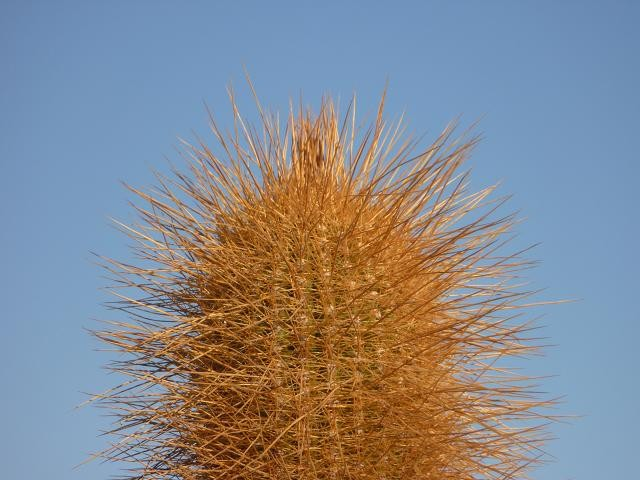
\includegraphics[width=4.8cm]{articles/La-paz-humahuaca-et-salaar/12572037289e7N.jpg}
Une montagne de cure dents.

\hspace*{-0.65cm}
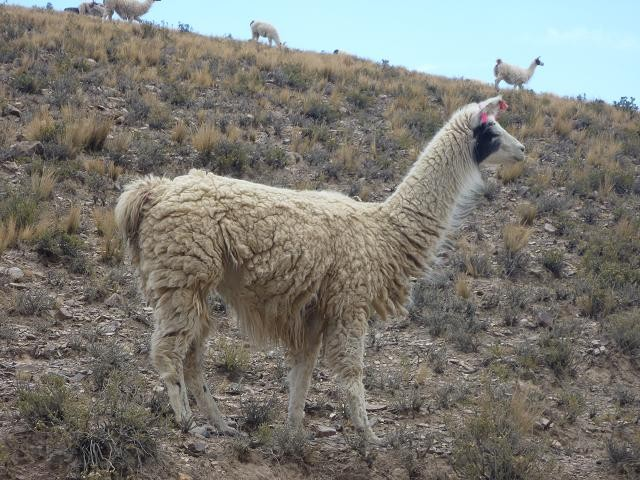
\includegraphics[width=4.8cm]{articles/La-paz-humahuaca-et-salaar/1257387254hVhj.jpg}
Des alpagas.

\hspace*{-0.65cm}
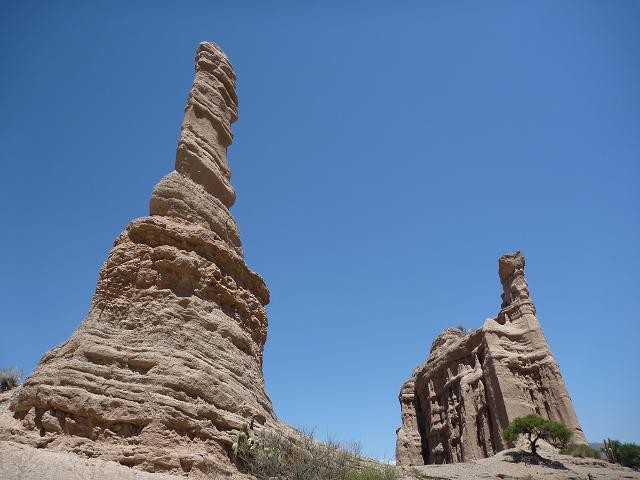
\includegraphics[width=4.8cm]{articles/La-paz-humahuaca-et-salaar/1257387285NQRd.jpg}
Formations rocheuses sur la route du Salaar.

Le Salaar, que dire, 12.000 kilomètres carrés d'étendue de sel, plat à perte de vue, pleins de petits octogones formes je ne sais comment, c'est tout simplement magnifique.

L'hôtel de sel.

\hspace*{-0.65cm}
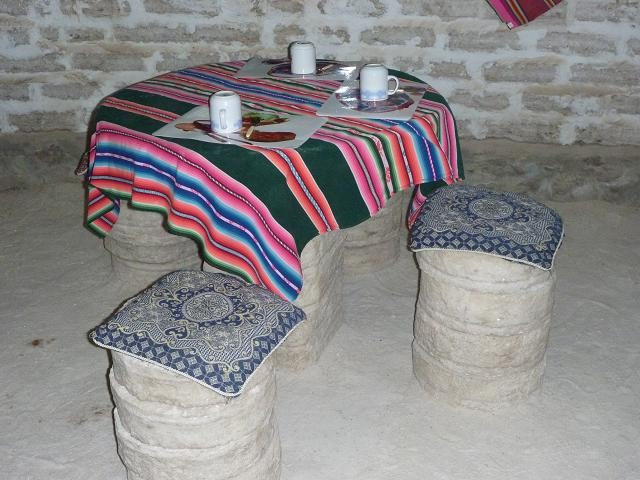
\includegraphics[width=4.8cm]{articles/La-paz-humahuaca-et-salaar/12573872732dVv.jpg}
Quand on a du sel sous la main, pourquoi tuiliser des briques ?

Voici une photo de nous trois au lever du soleil.

\hspace*{-0.65cm}
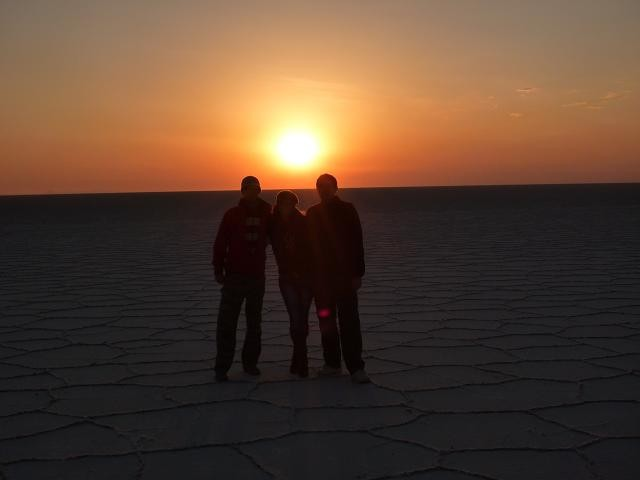
\includegraphics[width=4.8cm]{articles/La-paz-humahuaca-et-salaar/1257203731jBS0.jpg}
Lever de soleil dans le Salaar.

\hspace*{-0.65cm}
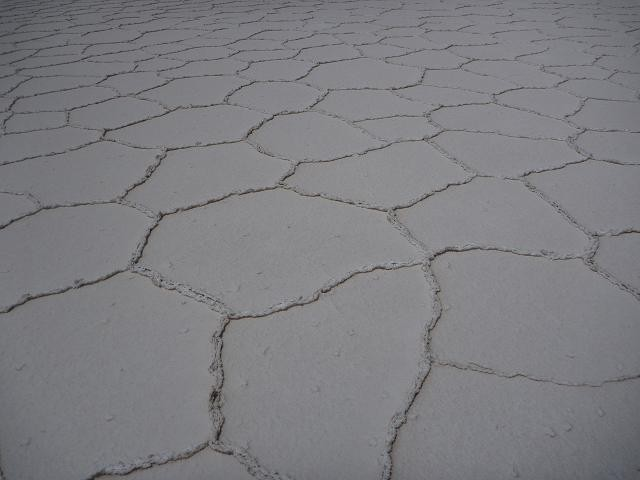
\includegraphics[width=4.8cm]{articles/La-paz-humahuaca-et-salaar/1257389754e5dq.jpg}
Détail du Salaar.

On y a passé des heures, et même fait un match de foot sur le sel.

\hspace*{-0.65cm}
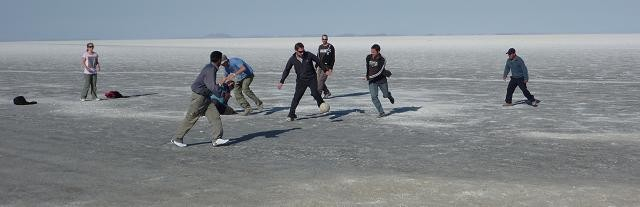
\includegraphics[width=4.8cm]{articles/La-paz-humahuaca-et-salaar/12573870691BvG.jpg}
Partie de foot.

Et à ce moment la, voyez qui on voit débarquer...

\hspace*{-0.65cm}
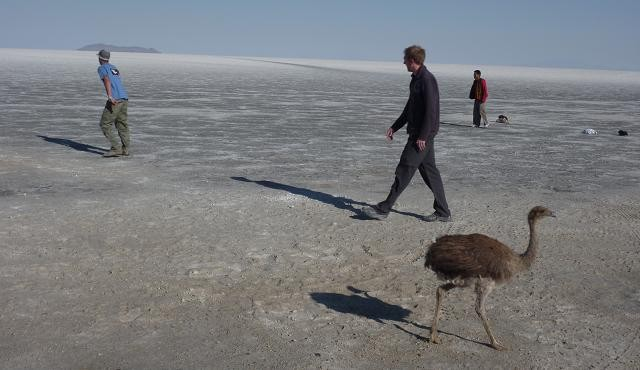
\includegraphics[width=4.8cm]{articles/La-paz-humahuaca-et-salaar/1257387056akBO.jpg}
Et un joueur de plus, un !

C'était vraiment super le Salaar, enfin jusqu'à ce que Luana ait faim, à ce moment on a vraiment failli y passer avec Neil, jugez plutot..

\hspace*{-0.65cm}
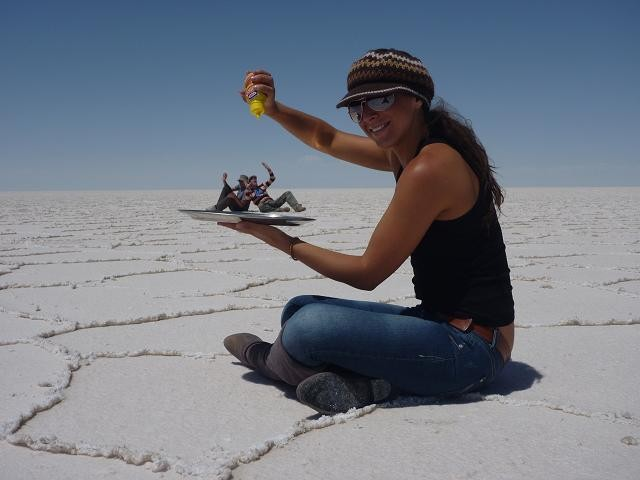
\includegraphics[width=4.8cm]{articles/La-paz-humahuaca-et-salaar/12572036252qaK.jpg}
Au secours, aidez nous...

Puis c'est finit pour le Salaar, le guide me laisse à Uyuni et renmène les deux autres lurons à Tupiza. J'attend deux heures du mat' pour prendre un train direction Oruro, mon plan est alors de voir sur place ce que je fait, où je vais et tout et tout. Nous arrivons à Oruro, 9h du matin. Deux heures avant je me suis aperçu que mon sac avait été ouvert dans la nuit, sans savoir ce qui avait disparu, j'ai alors pensé que c'était moi qui avait oublié de le refermer avant de m'endormir, même si c'est typiquement le genre de truc auquel je fait super gaffe, ça m'étonne donc de moi. Une fois à Oruro je cherche mon Lonely Planet pour planifier un peu ce que je fait à partir des 5 prochaines minutes et là je me rend compte que c'est ça qui a disparu. La stupidité de ce vol me fait encore rire. Un Bolivien, parlant castillan qui s'en va voler un guide touristique de son pays écrit en Français.. j'aurai payé cher pour voir sa tête quand il s'est rendu compte de ce qu'il avait pris..

Bon, ben moi je vais fair une petit tour dans la ville, Oruro est principalement connue pour son carnaval annuel, mais bon comme c'est pas maintenant ça me fait une belle jambe.. il faudra revenir. Un peu plus tard je prend un bus pour Cochabamba, plus à l'Ouest, moins arride. Cochabamba sera le début de l'article suivant. Je vous laisse donc ici. Mes plans pour la fin de mon voyage sont assez simples. Je pense repasser par La Paz pour acheter quelques trucs, puis aller à Cusco, au Pérou pour gravir le Machu Pichu et voir ses ruines Inca. Alors sonnera la fin du voyage, je rentrerai à Lima un ou deux jours en avance par rapport à mon avion pour parer tout retard de bus.

A très bientôt, et continuez de me lire assiduement jusque la fin, je vous promet un article avec pleins de photos une fois rentré en France.

Hasta la proxima..

\end{multicols}

\bigskip
\textbf{\textsc{Commentaires}}

\medskip
Tatid a écrit le 05 nov. 2009 :
\begin{displayquote}
Qu'est-ce que tu me fais rire avec tes histoires de fous ! C'est énorme ! On est à des années lumières de mes vacs aux USA lol !

Continue bien el gringo !

A plutch' !
\end{displayquote}

\medskip
Etienne a écrit le 06 nov. 2009 :
\begin{displayquote}
Et encore.. Je n'en raconte qu'une petite partie. Aujourd'hui je suis alle me perdre au dehors de Cochabamba en enchainant les collectivos, puis j'ai passe l'apres midi chez un imprimeur a discuter pendant que je le regardait faire tous ses reglages de machines. On est a mi chemin entre Gutenberg et le numerique, c'etait pitoresque, et super sympa.
\end{displayquote}

\medskip
Jaco a écrit le 07 nov. 2009 :
\begin{displayquote}
En tout cas super sympa la photo en "trompe l'oeil", elle m'a bien fait marrer :)
\end{displayquote}

\medskip
Titou et Chachou a écrit le 07 nov. 2009 :
\begin{displayquote}
Coucou,

Content d'avoir de tes nouvelles. On a eu du mal à les découvrir vu qu'on était resté sur la page PEROU... Ça a l'air vraiment génial ce que tu fais. On attend les détails à ton retour autour d'une bonne biere.

Profite bien de la fin de tes vacances et a très bientôt.

Bisous
\end{displayquote}

\medskip
Sonia a écrit le 08 nov. 2009 :
\begin{displayquote}
Et bien t'en vis des aventures!!... mais ça va? tu n'as pas eu trop peur qu'elle vous mange! lol

OK assidue jusqu'à la fin.

a bientôt
\end{displayquote}

\medskip
Didier a écrit le 10 nov. 2009 :
\begin{displayquote}
Tout bon tout bon tout ca vieux. Bon je t'attends le 10 au soir ici a Cuzco pour une bonne ptite soiree.

A toute
Didier le belge
\end{displayquote}

\medskip
Etienne a écrit le 13 nov. 2009 :
\begin{displayquote}
Youhouh.. je suis a l'arret au port, j'ai pas encore regarde si l'avion y est lui aussi mais y a pas de raison..
Finit les vacances, je reviens avec tout plein de trucs a dire, des photos a vous montrer.. alors a bientot pour un dernier post sur ce blog, avant le prochain voyage bien entendu, je ne m'arreterai pas la.

Muchos besos
\end{displayquote}

\medskip
Jaco a écrit le 10 janv. 2010 :
\begin{displayquote}
"alors a bientot pour un dernier post sur ce blog"

Alors ????
\end{displayquote}

\medskip
Sylvain a écrit le 28 juil. 2010 :
\begin{displayquote}
Bonjour,
Je viens de découvrir votre blog. Il est vraiment sympa. Nous avons fait un tour du monde l'année dernière avec un copain et nous sommes un peu nostalgiques.
Nous avions aussi fait un site : www.voyageautourdumonde.fr. Nous aimerions faire un échange de liens avec votre site. Je vous propose d'ajouter un liens vers votre site dans notre page de liens. Si en échange vous pouviez faire de même ce serait super.
Est ce que cela vous intéresserait ?
A bientôt,
Sylvain
\end{displayquote}


